%!TeX root = Chapter_Method
\documentclass[../../CompleteThesis/Complete_1stDraft.tex]{subfiles}
\begin{document}
	
\begin{figure}
	\centering
	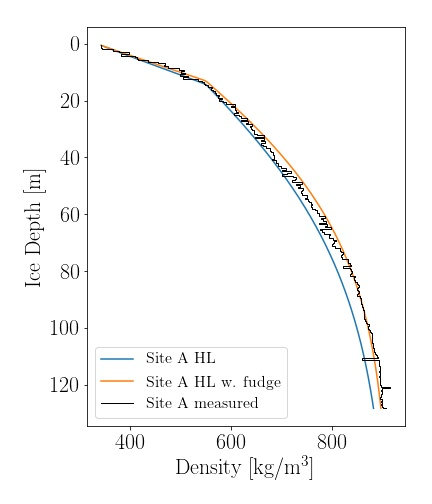
\includegraphics[width=0.7\textwidth]{SiteA_DensProfile_wHL.jpg}
	\caption[Density profile Site A]{Depth density profile at Site A. Black is the measured densities during drilling, blue is the modelled density profile given a Herron Langway model, and orange is a Herron Langway model with a criterion to minimize the distance to the actual measurements.}
	\label{Fig:SiteA_DensProfile_wHL}
\end{figure}

\begin{figure}
	\centering
	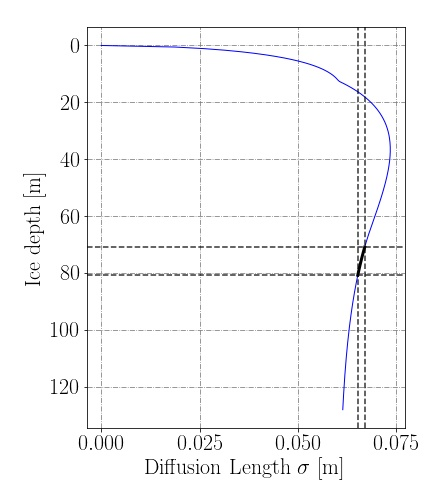
\includegraphics[width=0.7\textwidth]{SiteA_DiffProfile.jpg}
	\caption[Diffusion profile, Site A.]{Estimated diffusion profile at Site A given a Herron Langway model.}
	\label{fig:SiteADiffProfile}
\end{figure}

\begin{figure}
	\centering
	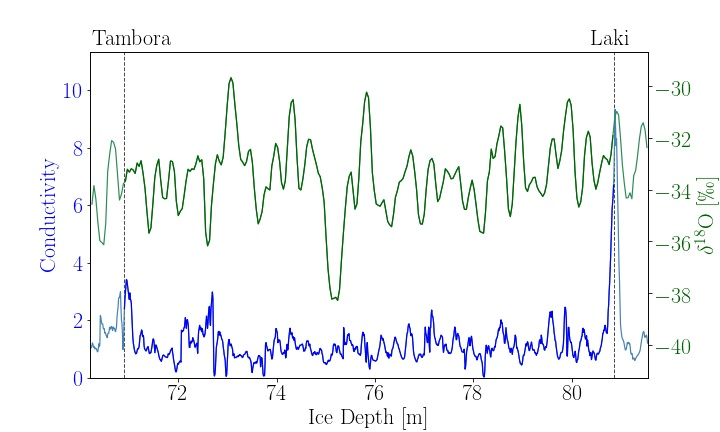
\includegraphics[width=0.9\textwidth]{SiteA_ECMd18O_combo.jpg}
	\caption[ECM and d18O data at LT, Site A.]{Two depth profiles from the core drilled at Site A showing accordingly the measured $\delta^{18}$O isotopic values and the conductivity measurements in the depth ranging from the estimated Tambora eruption to the Laki eruption.}	
	\label{fig:SiteA_ECMd18O_combo}
\end{figure}

\begin{figure}
	\centering
	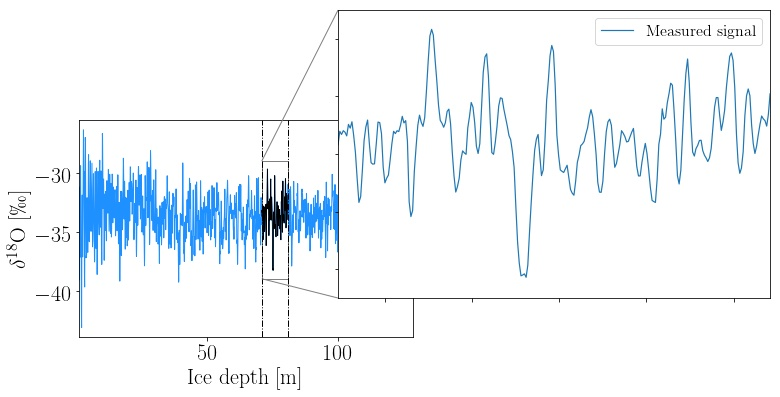
\includegraphics[width=0.9\textwidth]{SiteA_d18OInsert.jpg}
	\caption[Full $\delta^{18}$O record with insert, Site A]{The entire ice core isotopic profile from Site A, with a zoom in on the estimated depth series spanning from Tambora to Laki.}
	\label{fig:SiteA_d18OInsert}
\end{figure}

\begin{figure}
	\centering
	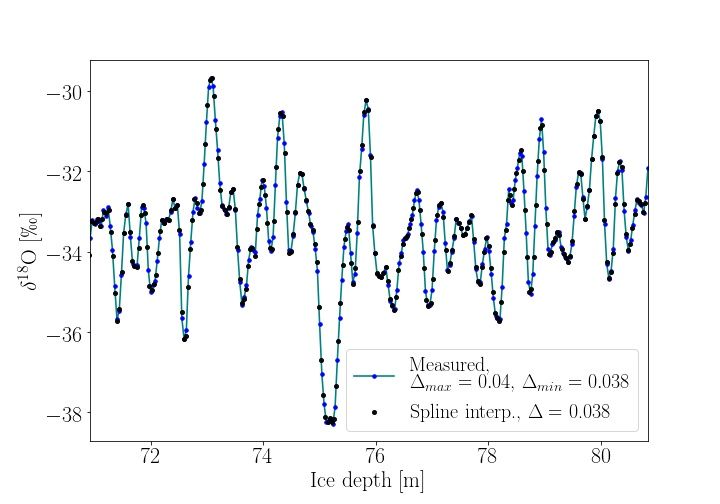
\includegraphics[width=0.9\textwidth]{SiteA_d18OLT_Interp.jpg}
	\caption[Measured and interpolated $\delta^{18}$O data, Site A]{The unevenly measured data from Site A in the depth ranging from Tambora to Laki along with the now evenly sampled cubic spline interpolated data. Sampled with an interval of $\Delta = 0.038$.}
	\label{fig:SiteA_d18OLT_Interp}
\end{figure}

\begin{figure}
	\centering
	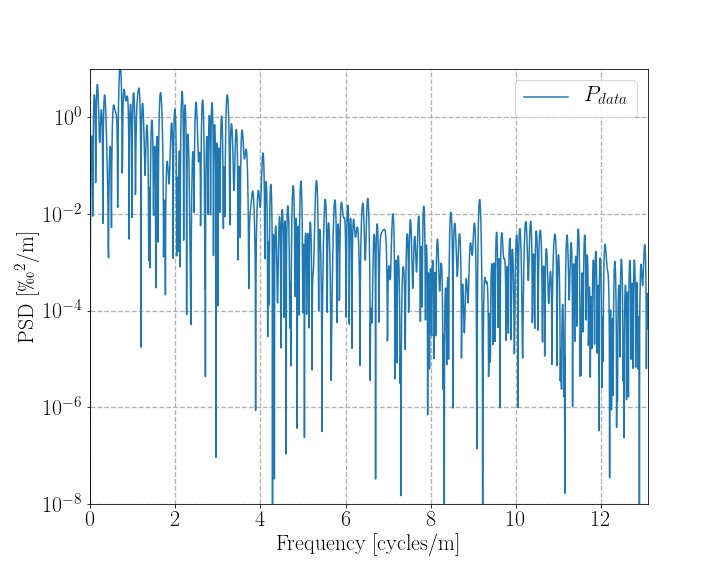
\includegraphics[width=0.9\textwidth]{SiteA_DCT_PSD_raw.jpg}
	\caption[PSD of LT data, Site A]{The power spectral density(PSD) of the interpolated data from Site A shown in Figure \ref{fig:SiteA_d18OLT_Interp}. The PSD was computed through a Discrete Cosine Transform(DCT).}
	\label{fig:SiteA_DCT_PSD_raw}
\end{figure}


\begin{figure}
	\centering
	\begin{subfigure}{.35\textwidth}
		\centering
		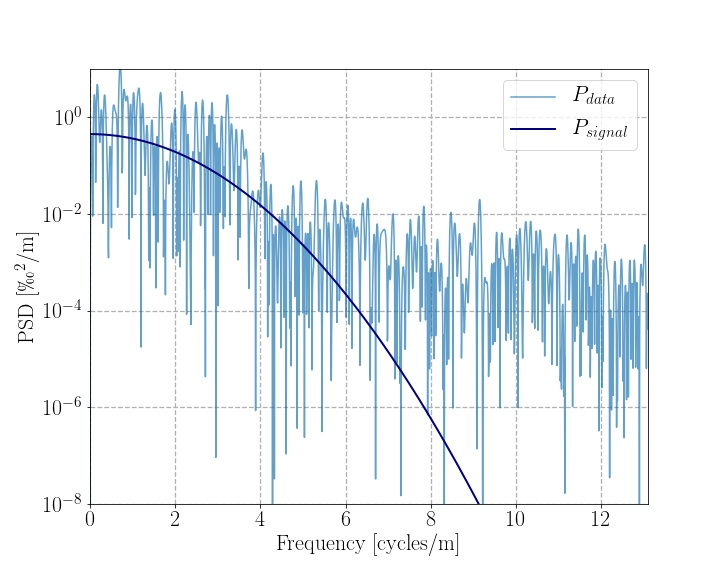
\includegraphics[width=\textwidth]{SiteA_PSD_sig.jpg}
		\caption{Signal estimate given through fitting to all data (noise and signal).}
		\label{fig:SiteA_PSD_sig}
	\end{subfigure}%
	~~~~
	\begin{subfigure}{.35\textwidth}
		\centering
		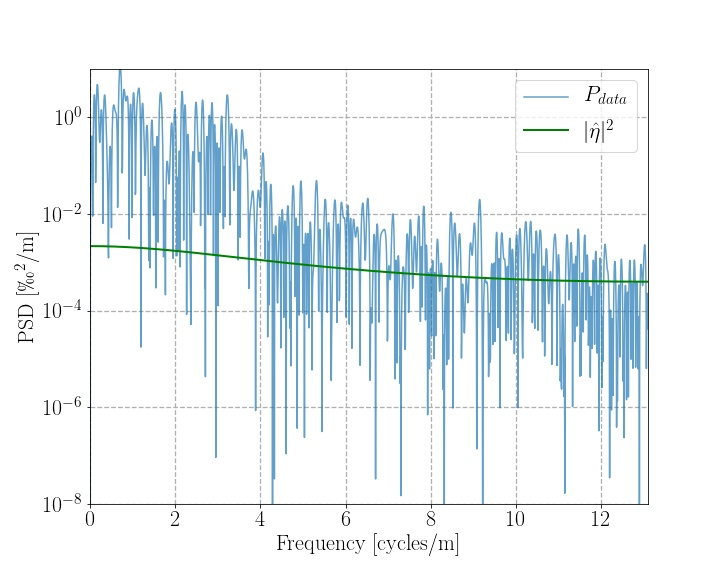
\includegraphics[width=\textwidth]{SiteA_PSD_noise.jpg}
		\caption{Noise estimate given through fitting to all data (noise and signal).}
		\label{fig:SiteA_PSD_noise}
	\end{subfigure}%
	~~~~
	\begin{subfigure}{.35\textwidth}
		\centering
		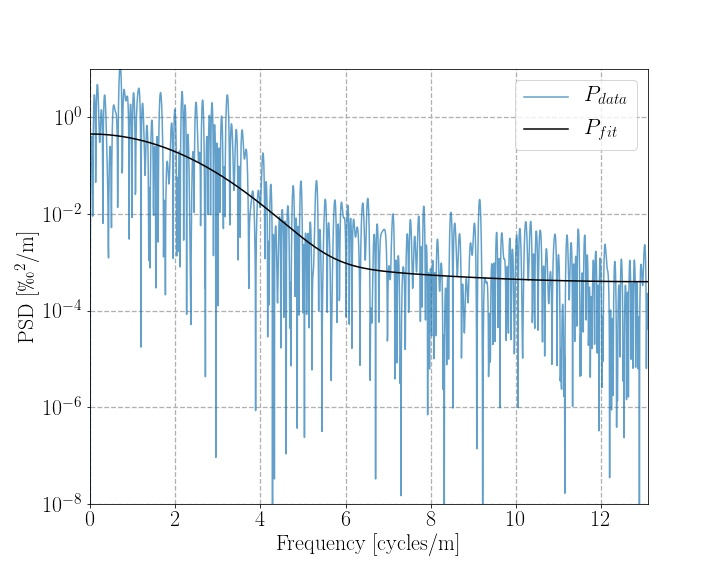
\includegraphics[width=\textwidth]{SiteA_PSD_fit.jpg}
		\caption{Complete spectral fit to all data (blue), both noise and signal.}
		\label{fig:SiteA_PSD_fit}
	\end{subfigure}\\[1ex]
	\begin{subfigure}{0.9\linewidth}
		\centering
		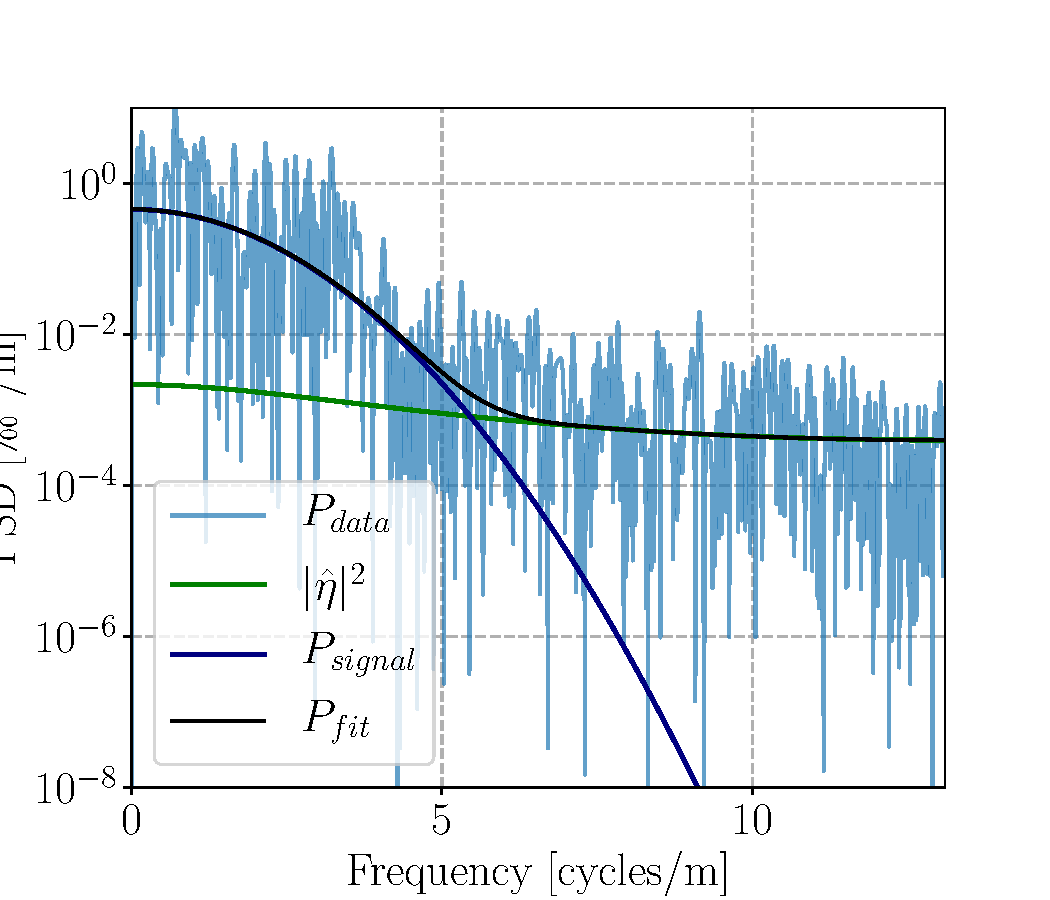
\includegraphics[width=\textwidth]{SiteA_PSD_all}
		\caption{Signal(blue) and noise(green) estimates through fit(black).}
		\label{fig:SiteA_PSD_all}
	\end{subfigure}
	\caption[Spectral fit, Site A]{Spectral estimate of the depth series from Tambora to Laki along with fit to entire spectral data set and the separated estimates of the noise and signal functions, as described in section \ref{sec:??}.}
	\label{fig:test}
\end{figure}




\begin{figure}
	\centering
	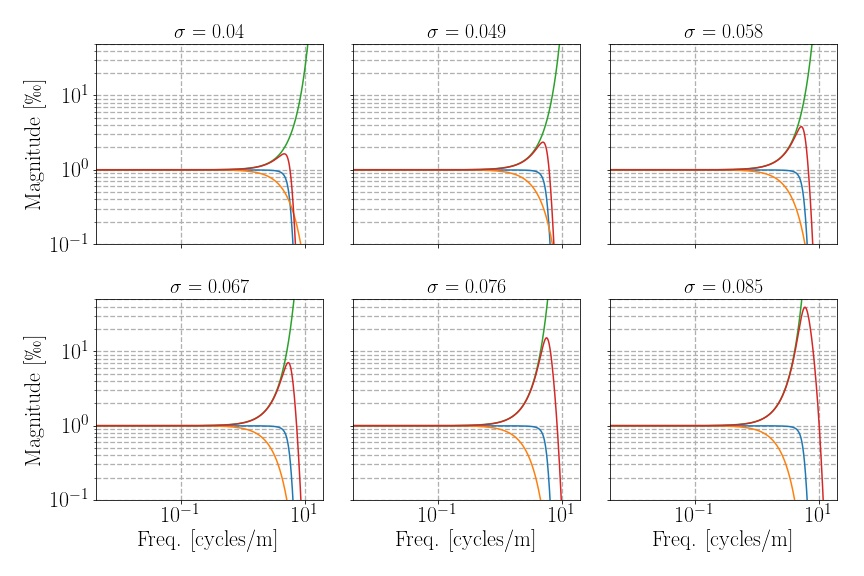
\includegraphics[width=0.9\textwidth]{SiteA_filtersEx.jpg}
	\caption[Frequency filters example, Site A]{Frequency filter examples ranging from diffusion length 0.04 m to 0.085 m.}
	\label{fig:SiteA_filtersEx}
\end{figure}

\begin{figure}
	\centering
	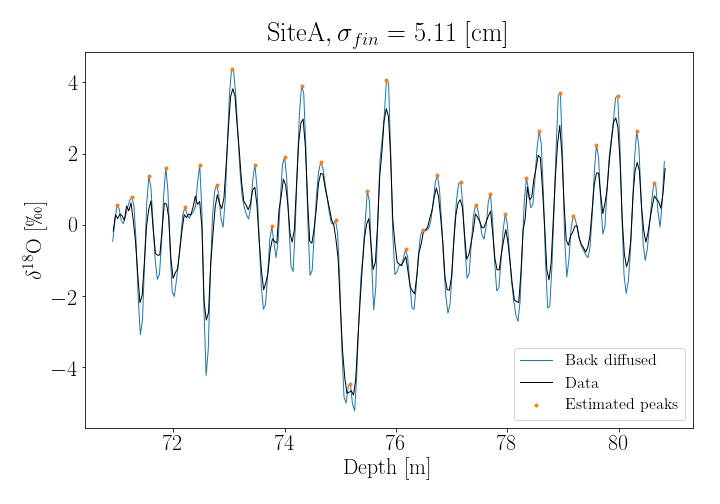
\includegraphics[width=0.9\textwidth]{SiteA_BackDiffused_Y32.jpg}
	\caption[Best estimate of deconvoluted depth series, Site A]{Best estimate of deconvoluted depth series given an annual count of 32 years - marked as orange dots. The best estimate is taken as the largest diffusion length that still yields 32 years in the depth span from Tambora to Laki.}
	\label{fig:SiteA_BackDiffused_Y32}
\end{figure}

\begin{figure}
	\centering
	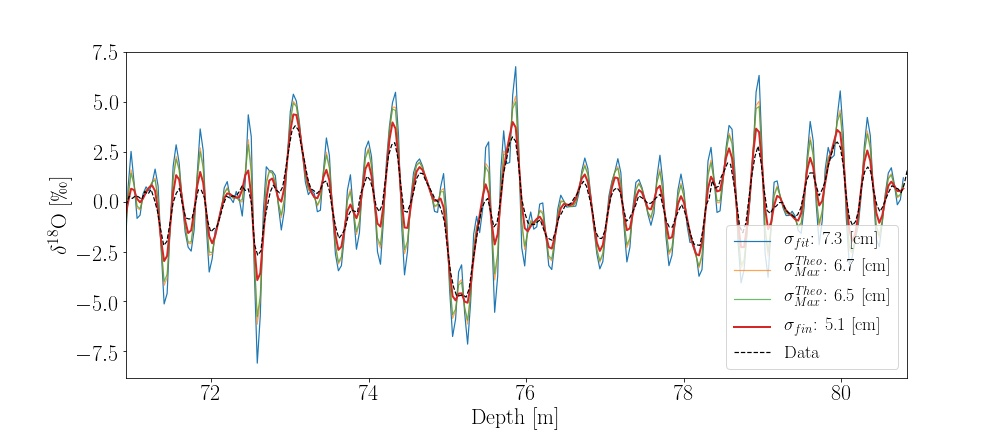
\includegraphics[width=\textwidth]{SiteA_BackDiffused_AllSigmaEst.jpg}
	\caption[All diffusion length estimate deconvolutions, Site A]{Estimated back diffused data series with different diffusion length estimates: diffusion length estimate from spectral fit ($\sigma_{fit}$), maximum ($\sigma_{Max}^{Theo}$) and minimum ($\sigma_{Min}^{Theo}$) theoretically estimated diffusion lengths and final estimated diffusion length.}
	\label{fig:SiteA_BackDiffused_AllSigmaEst}
\end{figure}


\end{document}
